% ---------------------------------------------------------------------------
\section{Comparisons}
\label{sec:comparisons}

\subsection{Natural and constructed languages}

Table~\ref{tab:languages} and Figure~\ref{fig:languages} compare the Voynich with the 24 natural languages, one value
per language (\expcode{e3c84}). Version~1 compared it with ``71 languages'', which were in fact 71 texts, some of them in
constructed languages, and two of the reported maxima came from Toki Pona. Summarised per natural language, the
statements of version~1 that the Voynich lies beyond all languages hold for the attested wrong cuts, the mirroring of
within-word rules, the frequency--form correlation and the two repetition rates; spaces and form filling are exceeded
only by Chinese in pinyin, whose words are syllables; the junction is exceeded by Sanskrit and Tagalog; margin avoidance
by Portuguese. Section~\ref{sec:boundaries} shows that four of these properties follow from word form; the comparison
says how unusual the word form is, not that the text is a chain.

\begin{table}[htbp]
\centering\footnotesize
\caption{The Voynich against the 24 natural languages of \citet{gaskellbowern2022}, one value per language (median of
its texts; first 10{,}000 words), and against the constructed languages. ``Beyond'' counts the languages further than the
Voynich in its own direction; the sensitivity columns use language and period, and the text of each language closest to
the Voynich. Experiment \expcode{e3c84}.}
\label{tab:languages}
\begin{tabularx}{\linewidth}{>{\raggedright\arraybackslash}p{3.6cm}r>{\centering\arraybackslash}X>{\centering\arraybackslash}X>{\centering\arraybackslash}p{2.0cm}}
\toprule
measure & Voynich & languages: median (range) & languages beyond: per language / period / closest text & constructed beyond \\
\midrule
F1 of spaces from the two flanking glyphs & 0.862 & 0.644 (0.520--0.951) & 1 / 1 / 1 & none \\
form filling & 0.434 & 0.046 (0.016--0.465) & 1 / 1 / 1 & none \\
attested wrong cuts & 0.499 & 0.065 (0.037--0.236) & 0 / 0 / 0 & none \\
mirroring of within-word rules ($\rho$) & 0.470 & 0.030 ($-0.252$--0.371) & 0 / 0 / 0 & none \\
frequency follows form ($\rho$) & 0.583 & 0.087 ($-0.018$--0.260) & 0 / 0 / 0 & none \\
junction (bits) & 0.191 & 0.097 (0.034--0.220) & 2 / 3 / 4 & none \\
identical neighbours & 1.01\% & 0.13\% (0.01--0.40\%) & 0 / 0 / 0 & none \\
near-identical neighbours & 4.13\% & 0.25\% (0.06--1.86\%) & 0 / 0 / 0 & none \\
left margin (observed/expected) & 0.51 & 0.97 (0.42--1.35) & 1 of 23 & Lojban \\
repetition decline within the line & 0.12 & 2.86 ($-3.89$--12.85) & 2 of 20 & Lojban, Toki Pona \\
\bottomrule
\end{tabularx}
\end{table}

\begin{figure}[htbp]
\centering
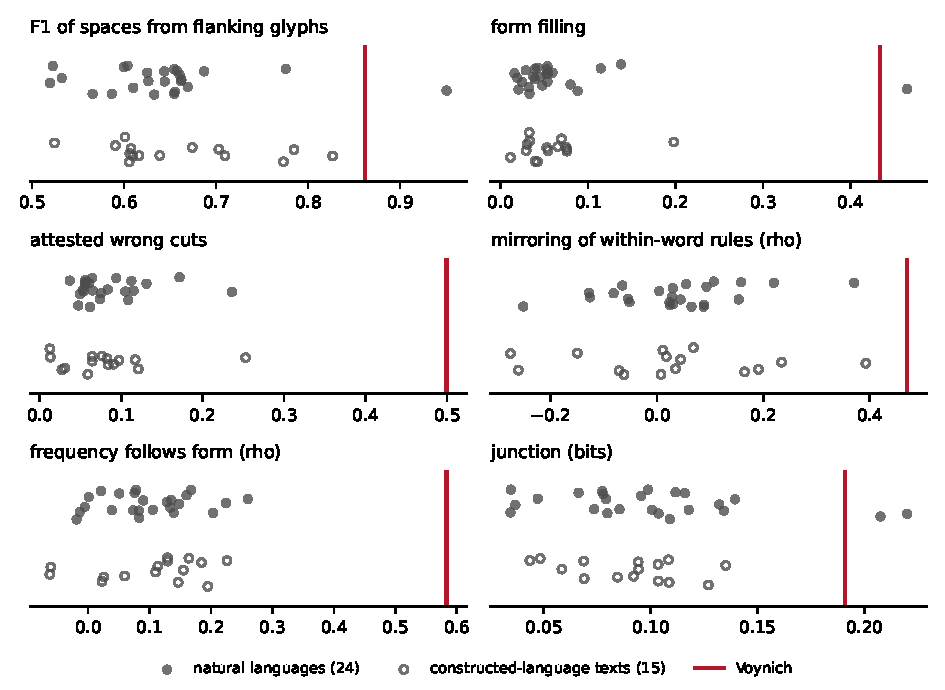
\includegraphics[width=\linewidth]{figure/lingue.pdf}
\caption{The Voynich (red line) among the 24 natural languages (dots, one per language) and the constructed languages
(open circles) for six measures. Data: \expcode{e3c84}.}
\label{fig:languages}
\end{figure}

\subsection{Seventy-nine medieval manuscripts and a cipher copyist}
\label{sec:scribes}

If the rules of Section~\ref{sec:rules} were ordinary scribal habits, real scribes copying real texts would have them.
We measured the same properties, with the same code, in 79 manuscripts transcribed at the level of letter forms with
their original lines and pages: six Nordic manuscripts from about 1200 to 1550 \citep{menota} and 73 German manuscripts
from 1350 to 1500, the area and century of the Voynich, with lines of five to eight words \citep{ref2021}. A variant
choice was measured only if it occurs at least 300 times in its minority form among words that show both forms; this
rule excludes the choices that are fixed by position in the word (for example a long \emph{s} that never appears at the
end). Table~\ref{tab:battery} gives the results and Figure~\ref{fig:battery} the intervals choice by choice.

\begin{table}[htbp]
\centering\footnotesize
\caption{The scribe battery: properties of the Voynich measured identically in 79 medieval manuscripts and in the
Copiale. ``Absent with power'' means that the upper end of the 95\% interval lies below half the Voynich value
(\expcode{e3c90}).}
\label{tab:battery}
\begin{tabularx}{\linewidth}{>{\raggedright\arraybackslash}p{2.8cm}YYYYY}
\toprule
property & Voynich & 6 Nordic manuscripts & 73 German manuscripts & Copiale copyist & reading \\
\midrule
junction rule (effect / uncertainty of the choice) & 0.058 & 2 of 11 choices at 0.013--0.015, others zero & 2 of 13 at
0.001--0.005, others zero & --- & about 4 times the strongest Nordic choice, 12 times the strongest German one \\
left margin: avoiding the start of the line above & 5 starts avoided & none in 72 tests & no manuscript with 3 or more
starts avoided; 3 of 72 with one, as expected by chance & --- & not found in the manuscripts \\
line-edge forms (gain of the most typical form) & end \eva{-m} $+0.151$; start \eva{s-} $+0.098$ & $+0.016$ to $+0.025$
(abbreviations at line end, \eva{v-} at start) & $+0.019$ (line-break hyphen); $+0.012$ & --- & same kind, 4--8 times
stronger in the Voynich \\
immediate repetition, observed/expected within the line & 1.04 & 0.02--0.07 & at most 0.79 & 0 & avoided by every scribe,
not by the Voynich \\
drift along the line (per 10 glyphs) & $-0.020$ to $-0.034$ & at most 0.0075 & at most 0.008, in no common direction &
--- & no choice drifts as much; absent with power in 20 of 29 choices \\
short state of choices, at 2--3 words & $+0.09$ & \multicolumn{2}{p{5.2cm}}{absent with power in 14 of 29 choices;
not measurable in 13; present in 2: AM 302 fol \emph{ſ/s} ($+0.08$, from copying similar words) and Holm A 10
round/straight \emph{r} ($+0.05$, also between different words; uncertain)} & \textbf{rotates} homophones: $-0.18$ between adjacent
words & weaker or absent in scribes; not established as unique \\
slow state between consecutive lines & $+0.050$ & 6 of 17 choices, 5 as large as the Voynich & --- & --- & normal in
handwriting \\
\bottomrule
\end{tabularx}
\end{table}

\begin{figure}[htbp]
\centering
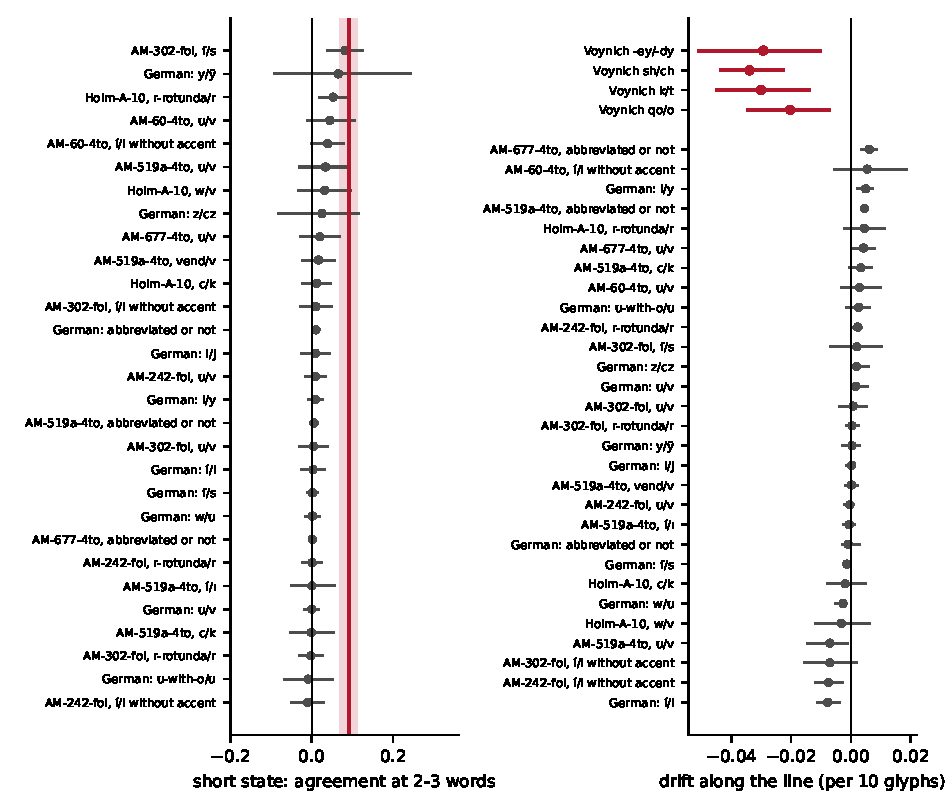
\includegraphics[width=\linewidth]{figure/scribi.pdf}
\caption{Short state (agreement at two and three words, left) and drift along the line (right) in each choice of the 79
manuscripts, with 95\% intervals, against the Voynich (red band: its 95\% interval by bifolium). Choices of the German
manuscripts are measured on the 73 manuscripts together. Data: \expcode{e3c50}, \expcode{e3c58}, \expcode{e3c62},
\expcode{e3c77}, \expcode{e3c86}, \expcode{e3c90}.}
\label{fig:battery}
\end{figure}

\paragraph{What it means} Junction rules, left-margin avoidance and the non-avoidance of immediate repetition have no
counterpart in these manuscripts; line-edge forms exist in scribes but are four to eight times weaker; the drift is
smaller in every choice (at most 0.008 against 0.020--0.034 per ten glyphs) and absent with adequate power in 20 of 29.
The short state is the property for which the comparison is weakest:
with the data available it can be called absent in only half of the choices, and the Swedish scribe of Holm A 10 shows,
in the choice between round and straight \emph{r}, an agreement half as large as the Voynich's that holds between
different words too (\expcode{e3c91}, uncertain). The slow state is normal in handwriting. The Copiale copyist does the
opposite of the Voynich: having used one symbol for a letter, he tends to use another in the next word (agreement
$-0.18$, down to $-0.48$ for \emph{u}), as one would expect from someone rotating homophones. Fifteenth-century German
herbals, recipe books and astrology texts written by hand repeat the adjacent word 7 to 30 times less than the Voynich,
so repetition does not come from genre.

These conclusions concern Old Norse and Early New High German manuscripts. Latin or Italian manuscripts of the fifteenth
century transcribed at the level of letter forms, the closest in place and kind to the Voynich, are not in the battery.

\subsection{Ciphers, readings and generators}
\label{sec:ciphers}

Every negative result in this subsection comes from a test that recovers the answer when it is there (positive control).

\paragraph{Encodings of real texts} We encoded real texts (Latin, Italian, the Bible, technical texts) and measured
whether they acquire the properties of the Voynich. A word-for-word code takes the letters and the vocabulary of the
Voynich but not its repetitions, page homogeneity or junction rules. Verbose ciphers in which each letter becomes a group
of two or three glyphs (450 variants) do not reach the predictability of the Voynich with words of its length. The
Naibbe cipher, in which each letter or pair of letters becomes a whole word chosen from homophonic tables, does: its
predictability and word length are close to the Voynich's, and \citet{kinnison2026} shows that it reproduces the
positional entropy profile. It does not reproduce repetitions, unique words, page homogeneity, the junction (almost zero)
or the line properties. Abbreviations, null letters and transpositions move away from the Voynich; encoded lists,
prayers and litanies take on its grain but not its anomalies.

\paragraph{Substitution readings} Homophonic substitution with spaces in 14 languages recovers 69--98\% of the words of
the controls and at most 36\% of Voynich ``words'', mostly the same three. A solver without spaces (simulated annealing
on a five-gram model of Latin trained on nine million letters, recovering 98--100\% of the keys of its positive
controls) never reliably beats the negative controls on the Voynich, whatever the glyph inventory, the grouping or the
reading direction. Further tests (85 languages with spaces; 16 vernaculars, historical languages and abbreviated Latin;
a mixed nomenclator; searches guided by plant names and months; other reading orders; pieces of words as symbols) gave
no reading; two formally positive outcomes proved to be artefacts. The order of glyphs inside words is language-like,
not anagram-like \citep[compare][]{hauerkondrak2016}.

\paragraph{Published readings} \citet{bax2014}: his recurring words do not behave as names (\eva{shor}, read as
``black'', occurs 96 times on 67 pages of all sections), and against 10{,}000 random keys his key does not beat chance on
the pages not used to build it ($p = 0.14$). \citet{vatne2021}: the reading relies on a transcription of its own; for
the 28 of 84 entries that match the reference transliteration, the claim that these words occur nowhere else is false (12
occur on other pages, as often as other paragraph-initial words); the other two thirds could not be tested.
\citet{cheshire2019}: the key reads more Romance words than chance, but any key of the same form adapted to the
manuscript does better, also on pages not used to adapt it (20 keys of 20). \citet{schechter2026}: the program,
re-implemented, gives the published figures, but a ``glossary'' of the most frequent words without any meaning covers as
much, the glossary ``reads'' 67--70\% of a text without a message, and the decoded word order is not Latin.
\citet{gatta2026}: the signal is equally present in a text without a message, and a mapping searched for on purpose does
better; the current version of the work itself concludes that the text does not behave like Hebrew. Applying a reading
to a text generated without content is simple, and we propose it as a minimum test for any announced decipherment.

\paragraph{Historical mechanisms} We looked for the signature that some encryption systems would leave, after checking on
texts enciphered on purpose that each test sees it. Several of these mechanisms are later than the vellum, so these are
tests of a kind of mechanism, not historical hypotheses. Homophones chosen by the copyist, as in the Copiale, would leave
a negative agreement between nearby words; the Voynich has a positive one. No frequent word or sign behaves like the
index letters of Alberti's cipher disk \citep[c.~1466;][]{alberti1466}. A message in the binary choices, as in Bacon's
biliteral cipher \citep{bacon1623}, restarting at each page or line, would be seen with overwhelming evidence ($z$ up to
70 in the controls) and is absent; a continuous message is out of reach of the test. The word tables of
\citet{trithemius1518} leave no rhythm of two to six words. An autokey restarting at each line is the only mechanism
tested that closes the line like the Voynich, but it destroys repetition, inflates the vocabulary (4{,}500--6{,}400
distinct words per 10{,}000, against 2{,}900) and leaves no margin avoidance.

\paragraph{Constructed languages, gibberish and generators} No constructed language has the junction rules, the line
properties or an agreement between adjacent word forms like the Voynich's. The volunteers' gibberish has no junction
(0.014), no line-edge forms, no copying from the line above and no margin avoidance (it repeats line starts). Among the
published generators we measured, Naibbe has neither junction nor line properties; the generator of
\citet{timmschinner2020} copies from too far above, has no junction closed within the line, no word-independent state,
no margin avoidance and no drift; U2 and U3 \citep{whitehatnetizen2026} do not combine the junction with a closed line.
We have not run \emph{voynich-fingerprint} \citep{sachak2026}, whose 44 statistics, reproduced on held-out folios, include
a cross-word junction computed without line breaks but no line-final forms, no vertical relation and no margin; our
statement is therefore limited to the generators measured.
